\chapter{THỰC NGHIỆM KẾT QUẢ VÀ ĐÁNH GIÁ}
Qua các chương trước, luận văn đã trình bày thuật toán, lý thuyết cũng như cách thức hoạt động của chương trình nhận dạng ngôn ngữ ký hiệu. Ở chương này, luận văn sẽ trình bày việc xây dựng ứng dụng nhận diện dựa trên mô hình đã huấn luyện, kết quả thực nghiệm mà luận văn đã đạt được sau khi huấn luyện và các phương pháp đánh giá độ chính xác của mô hình.
\section{Thực hiện phần mềm nhận dạng ngôn ngữ ký hiệu}
Tiếp theo, luận văn tiến hành xây dựng phần mềm nhận dạng thời gian thực để ứng dụng được mô hình đã huấn luyện trên ra thực tế. Việc xây dựng phần mềm ứng dụng này giúp người sử dụng có thể tương tác với ứng dụng thông qua nút bấm và chuột, làm chúng thân thiện với người dùng hơn.
\begin{itemize}
\item[$\square$] \textbf{Ngôn ngữ lập trình: }
Python được sử dụng làm ngôn ngữ lập trình chính để xây dựng model cũng như viết ứng dụng nhận dạng. Python là ngôn ngữ lập trình hướng đối tượng, cấp cao, mạnh mẽ, được tạo ra bởi Guido van Rossum. Python được sử dụng nhiều trong machine learning và deep learning bởi vì tính phổ biến và có rất nhiều thư viện hỗ trợ từ việc xử lý dữ liệu cho đến xây dựng mô hình machine learning như Tensorflow, Keras, Pandas, ...
\item[$\square$] \textbf{Thư viện Keras}
Thư viện Keras được sử dụng trong việc xây dựng model trong luận văn. Keras là một framework mã nguồn mở cho deep learning được viết bằng Python. Nó có thể chạy trên nền của các deep learning framework khác như: tensorflow, theano, CNTK. Với các API bậc cao, dễ sử dụng, dễ mở rộng, keras giúp người dùng xây dựng các deep learning model một cách đơn giản. Keras có một số ưu điểm như :

	\begin{itemize}
	\item Dễ sử dụng,xây dựng model nhanh.
	\item Có thể run trên cả cpu và gpu
	\item Hỗ trợ xây dựng CNN , RNN và có thể kết hợp cả 2.
	\end{itemize}
\end{itemize}

\FloatBarrier
\begin{figure}[htp]
\begin{center}

\includegraphics[scale=0.5]{chap6/c6_figs/keras.png}
\end{center}
\caption{Thư viện hỗ trợ Keras}
\label{fig:keras}
\end{figure}
\FloatBarrier

Chương trình nhận dạng được xây dựng trên hệ điều hành ubuntu, sử dụng camera là webcam. Giao diện được viết trên thư viện PyQt5, là một thư viện hỗ trợ viết giao diện ứng dụng trên ngôn ngữ Python. Các nút điều khiển trên giao diện, giúp chọn các chế độ hoạt động của chương trình. Có tất cả 3 chế độ đều có thể hoạt động khi có nhiều người trong khung hình:
\begin{itemize}
\item Skeleton detection: Phát hiện và và trích đặc trưng khung xương từ camera.
\item Tracking: Theo dõi và đánh chỉ số của từng người trong khung hình dựa trên giải thuật Deep Sort.
\item Recognize: Theo dõi, đánh chỉ số từng người và nhận dạng ngôn ngữ ký hiệu.
\end{itemize}

\section{Kết quả}
Chương trình thực nghiệm đã nhận dạng được khá chính xác các hành động đã huấn luyện (16 ngôn ngữ ký hiệu) khi xử lý realtime. Tốc độ xử lý khá nhanh khi đạt được từ 8 -> 10 FPS. Giao diện và các mode hoạt động được trình bày như các hình \ref{fig:gui1}, \ref{fig:gui2}, \ref{fig:gui3}.

\FloatBarrier
\begin{figure}[htp]
\begin{center}
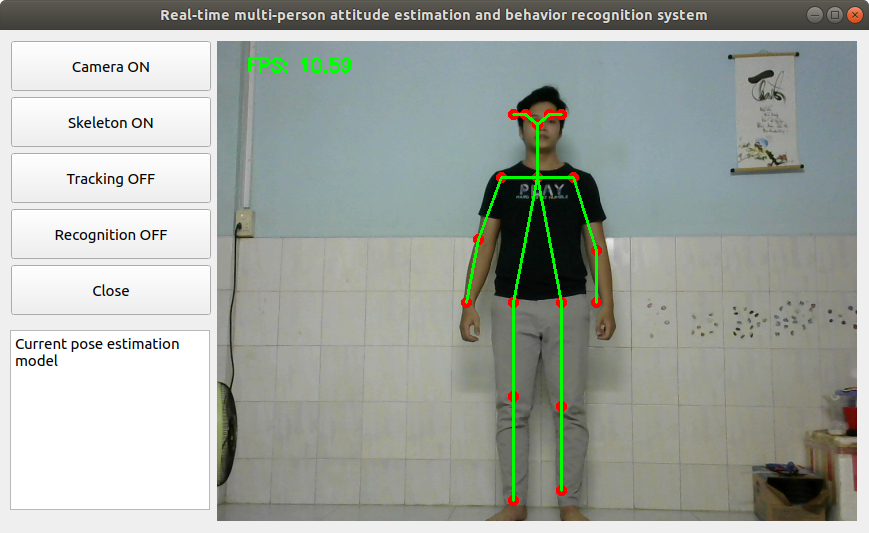
\includegraphics[scale=0.5]{chap6/c6_figs/mode_skeleton.png}
\end{center}
\caption{Giao diện phần mềm nhận dạng - Mode "Skeleton detection"}
\label{fig:gui1}
\end{figure}

\begin{figure}[htp]
\begin{center}
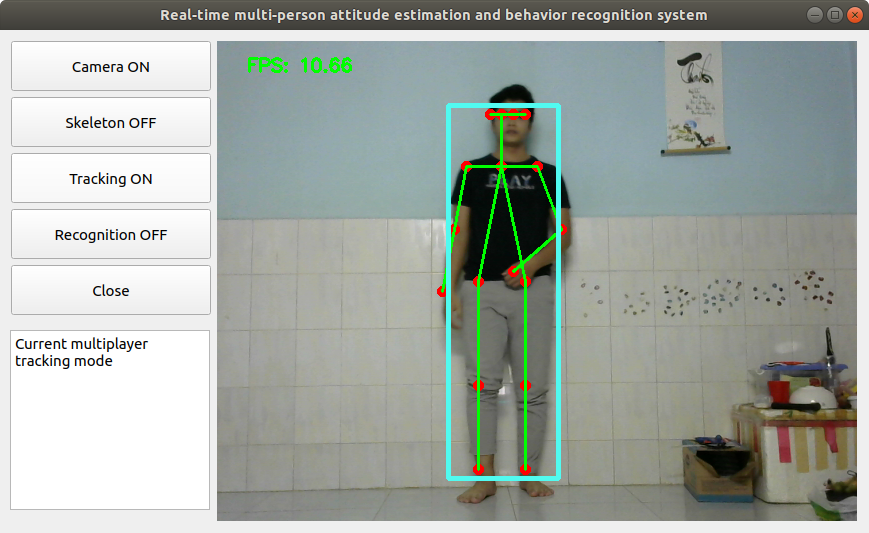
\includegraphics[scale=0.5]{chap6/c6_figs/mode_tracking.png}
\end{center}
\caption{Giao diện phần mềm nhận dạng - Mode "Tracking"}
\label{fig:gui2}
\end{figure}

\begin{figure}[htp]
\begin{center}
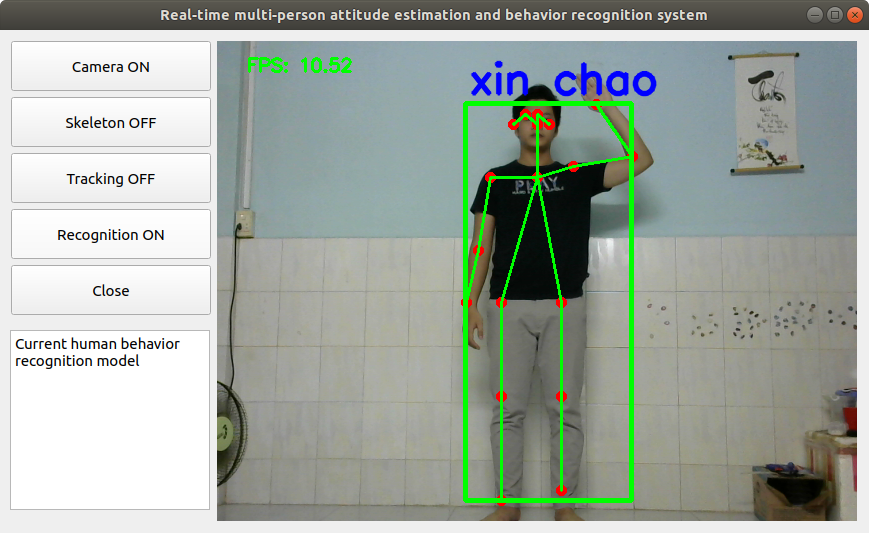
\includegraphics[scale=0.5]{chap6/c6_figs/mode_recognize.png}
\end{center}
\caption{Giao diện phần mềm nhận dạng - Mode "Recognize"}
\label{fig:gui3}
\end{figure}
\FloatBarrier

\section{Đánh giá}
Khi xây dựng một mô hình Machine Learning, chúng ta cần một phép đánh giá để xem mô hình sử dụng có hiệu quả không và để so sánh khả năng của các mô hình. Trong phần này, luận văn sẽ trình bày các mô hình classification.

Hiệu năng của một mô hình thường được đánh giá dựa trên tập dữ liệu kiểm thử (test data). Cụ thể, giả sử đầu ra của mô hình khi đầu vào là tập kiểm thử được mô tả bởi vector y\_pred - là vector dự đoán đầu ra với mỗi phần tử là class được dự đoán của một điểm dữ liệu trong tập kiểm thử. Ta cần so sánh giữa vector dự đoán y\_pred này với vector class thật của dữ liệu, được mô tả bởi vector y\_true. Đối với bài toán phân loại của luận văn, có 16 lớp dữ liệu được gán nhãn là tên các từ được huấn luyện.


Có rất nhiều cách đánh giá một mô hình phân lớp. Tuỳ vào những bài toán khác nhau mà chúng ta sử dụng các phương pháp khác nhau. Các phương pháp thường được sử dụng là: accuracy score, confusion matrix, ROC curve, Area Under the Curve, Precision and Recall, F1 score, Top R error, ...

Trong phần này, luận văn sẽ trình bày về phương pháp đánh giá sử dụng accuracy và confusion matrix. Sau đó đánh giá mô hình của luận văn trên tập dữ liệu test data gồm gần 150 SJM đối với mỗi từ.

\subsection{Accuracy}
Cách đơn giản và hay được sử dụng nhất là accuracy (độ chính xác). Cách đánh giá này đơn giản tính tỉ lệ giữa số điểm được dự đoán đúng và tổng số điểm trong tập dữ liệu kiểm thử.

Với bộ validation data, model đạt được accuracy = 0.9961
\subsection{Confusion Matrix}
Việc sử dụng accuracy như trên chỉ cho chúng ta biết được bao nhiêu phần trăm lượng dữ liệu được phân loại đúng mà không chỉ ra được cụ thể mỗi loại được phân loại như thế nào, lớp nào được phân loại đúng nhiều nhất, và dữ liệu thuộc lớp nào thường bị phân loại nhầm vào lớp khác. Ngoài ra đối với các bài toán thực tế nếu số lượng dữ liệu bị mất cân bằng giữa các lớp thì đại lượng accuracy chưa đủ ý nghĩa. Để có thể đánh giá được các giá trị này, chúng ta sử dụng một ma trận được gọi là confusion matrix.

Về cơ bản, confusion matrix thể hiện bao nhiêu điểm thực sự thuộc vào một class, và được dự đoán là rơi vào một class. Confusion matrix là một ma trận vuông với kích thước mỗi chiều bằng số lượng các lớp dữ liệu. Giá trị tại hàng thứ $i$, cột thứ $j$ là số lượng điểm lẽ ra thuộc class $i$ nhưng được dự đoán vào class $j$. Tổng các phần tử trong toàn ma trận chính là số điểm trong tập kiểm thử. Các phần tử trên đường chéo của ma trận là số điểm được phân loại đúng của mỗi lớp dữ liệu. Từ đây có thể suy ra accuracy chính bằng tổng các phần tử trên đường chéo chia cho tổng các phần tử của toàn ma trận. Đối với bài toán trong luận văn, confusion matrix được áp dụng trên tập dữ liệu test ta được kết quả như hình \ref{fig:confusion_matrix}.

\FloatBarrier
\begin{figure}[htp]
\begin{center}
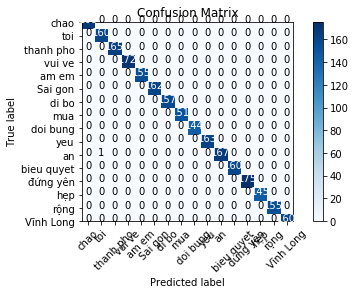
\includegraphics[scale=1]{chap6/c6_figs/confusion_matrix.png}
\end{center}
\caption{Confusion matrix của 16 lớp phân loại}
\label{fig:confusion_matrix}
\end{figure}
\FloatBarrier

Ta thấy rằng, confusion matrix mang nhiều thông tin hơn, giúp chúng ta xác định cụ thể model nhận diện kết quả với từng lớp như thế nào. Dựa vào confusion matrix \ref{fig:confusion_matrix} ta thấy mô hình đã nhận diện chính xác cao đối với từng lớp. Kết quả mô hình đã đạt được mục tiêu ban đầu của luận văn.